\documentclass[11pt]{article}
\usepackage[margin=1in]{geometry}
\usepackage{booktabs}
\usepackage{amsmath,amssymb}
\usepackage{graphicx}
\usepackage{xcolor}
\usepackage{hyperref}
\usepackage{enumitem}
\usepackage{tikz}
\usetikzlibrary{positioning,arrows.meta,fit,backgrounds}
\usepackage[round]{natbib}

\title{Model of Models: When Does Emitting a Specialist\\
Beat Attending, Adapting, or Tuning?\\[0.3em]
\large\normalfont A Controlled Cross-Domain Study of Amortized Weight Generation}
\author{John C. Howell\thanks{Nineonefour is the operating name of
Project[LNCLN]. Correspondence: \texttt{jc@nineonefour.org}.}\\
\small Nineonefour}
\date{\today}

\begin{document}
\maketitle

\begin{abstract}
We show that the weights a hypernetwork emits for a task-specific specialist are
\emph{algebraically composable}: linearly interpolating the weight vectors of two
emitted specialists yields a coherent blend of their functions---a circle-to-square
morph from $\theta_{\text{circle}}$ and $\theta_{\text{square}}$---a capability no
in-context or gradient-adaptation method possesses. We situate this within a broader
question: given a task described by a few examples, how should a model be specialized
to it? Four mechanisms are available---zero-shot, in-context attention, test-time
gradient adaptation, and emitting specialist weights---yet the operating regime of
the last is rarely mapped. We run the identical four-way comparison across six tasks
spanning regression, generation, language modeling, reinforcement learning, and
clinical and genomic classification, under matched budgets. Emitting specialists
dominates low-dimensional, amortizable task families: $380\times$ lower error than
MAML on few-shot sinusoid regression at \emph{zero} test-time gradient steps,
noise-floor shape generation at $840\times$ lower inference cost, and parity with the
state-of-the-art amortized tabular model (TabPFN) on clinical few-shot classification
while emitting a \emph{reusable} specialist rather than re-attending the support set
per query. It cannot match in-context attention on high-dimensional sequence
modeling, and the gap \emph{widens with scale}: a one-pass adapter captures only
$16\%$ then $11\%$ of the in-context gain as the base model grows from $5$M to $15$M
parameters. Mechanism ablations confirm the emitted specialist is genuinely
task-conditioned. We close with a falsifiable thesis bounding when each conditioning
mechanism should be preferred.
\end{abstract}

%==================================================================
\section{Introduction}

A recurring problem in machine learning is to specialize a general model to a
specific task that is described only by a handful of examples: a few labeled
patients, a few input--output grids, a few transitions from a new environment. Four
mechanisms are in common use. \emph{Zero-shot} ignores the examples. \emph{In-context}
learning prepends them and lets attention condition the forward pass. \emph{Gradient
adaptation}---MAML and ordinary fine-tuning---takes a few optimization steps on the
examples. The fourth, which we study here, \emph{emits} the parameters of a small
task-specific specialist network in a single forward pass of a hypernetwork. The
mechanism is not new: hypernetworks, conditional neural processes, and
context-to-LoRA generators all instantiate it. What is missing is a map of
\emph{when} it should be preferred over the other three.

We provide that map. We define a single formulation in which all four mechanisms
share a backbone and a budget (\S\ref{sec:method}, Fig.~\ref{fig:quadrant}) and run
the identical comparison across six tasks spanning five domains
(\S\ref{sec:exp}): few-shot sinusoid regression, parametric shape generation,
byte-level language modeling, meta-reinforcement learning, and clinical and genomic
few-shot classification. Rather than reporting only where emission wins, we
deliberately chart where it \emph{ties} and where it \emph{loses}, and we measure how
those boundaries move with scale.

Our most striking positive result is that emitted specialists are
\textbf{algebraically composable}: linearly interpolating the weight vectors of two
emitted specialists produces a coherent blend of their functions
(\S\ref{sec:compose}, Fig.~\ref{fig:morph})---a property no in-context or
gradient-adaptation method exhibits, and one that suggests the hypernetwork learns an
approximately linear map from task to weight space. Our most consequential negative
result is a scaling trend: on language modeling, a one-pass emitted adapter captures
a \emph{shrinking} fraction of the in-context performance gain as the base model
grows (\S\ref{sec:scaling}). Together they bound the method's regime.

\paragraph{Contributions.}
\begin{enumerate}[label=(C\arabic*),leftmargin=2.6em,topsep=2pt]
  \item A controlled four-way comparison of conditioning mechanisms across six tasks
        and five domains under matched budgets (\S\ref{sec:exp}).
  \item \textbf{Boundary maps} rather than wins: where emission dominates, ties, and
        loses---including a scaling trend in which the gap to in-context attention
        \emph{widens} for high-dimensional sequences (\S\ref{sec:scaling}).
  \item \textbf{Mechanism ablations} establishing that the emitted specialist is
        genuinely task-conditioned, not a memorized prior (\S\ref{sec:ablation}).
  \item \textbf{Weight-space composition}: emitted specialists interpolate and blend
        algebraically, including on a function family not closed under addition
        (\S\ref{sec:compose}).
\end{enumerate}

\paragraph{Thesis (falsifiable).} \emph{Amortized weight-emission dominates within a
trained low-dimensional task family, at far lower test-time cost than gradient
adaptation or in-context attention, but it cannot match in-context attention for
high-dimensional sequence modeling, and that gap grows with model scale.}

\begin{figure}[t]\centering
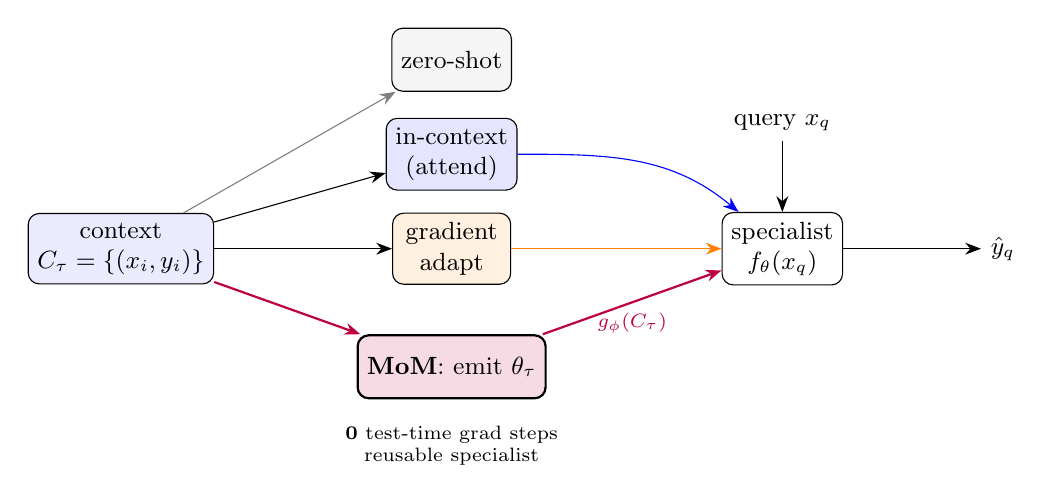
\begin{tikzpicture}[
  font=\small,
  box/.style={draw,rounded corners,minimum height=8mm,minimum width=15mm,align=center},
  ctx/.style={draw,fill=blue!8,rounded corners,minimum height=7mm,align=center},
  >={Stealth[length=2mm]}]
  % context
  \node[ctx] (c) at (0,0) {context\\$C_\tau=\{(x_i,y_i)\}$};
  % four mechanism rows
  \node[box,fill=gray!8] (zs) at (4.2,2.4) {zero-shot};
  \node[box,fill=blue!10] (ic) at (4.2,1.2) {in-context\\(attend)};
  \node[box,fill=orange!12] (ga) at (4.2,0.0) {gradient\\adapt};
  \node[box,fill=purple!14,thick] (mom) at (4.2,-1.5) {\textbf{MoM}: emit $\theta_\tau$};
  % shared specialist / query
  \node[box] (sp) at (8.4,-0.0) {specialist\\$f_{\theta}(x_q)$};
  \node (q) at (8.4,1.6) {query $x_q$};
  \node (yhat) at (11.2,-0.0) {$\hat y_q$};
  % arrows
  \draw[->,gray] (c) -- (zs);
  \draw[->] (c) -- (ic);
  \draw[->] (c) -- (ga);
  \draw[->,thick,purple] (c) -- (mom);
  \draw[->,thick,purple] (mom) -- node[below,font=\scriptsize]{$g_\phi(C_\tau)$} (sp);
  \draw[->,orange] (ga) -- (sp);
  \draw[->,blue] (ic) to[out=0,in=140] (sp);
  \draw[->] (q) -- (sp);
  \draw[->] (sp) -- (yhat);
  \node[font=\scriptsize,align=center] at (4.2,-2.5)
    {\textbf{0} test-time grad steps\\reusable specialist};
\end{tikzpicture}
\caption{The four conditioning mechanisms over a shared specialist $f_\theta$ and
query $x_q$. Zero-shot ignores the context; in-context attends to it every query;
gradient adaptation takes SGD steps on it; \textbf{MoM} emits the specialist's weights
$\theta_\tau=g_\phi(C_\tau)$ in one pass, with no test-time gradient steps and no
context in the query window.}
\label{fig:quadrant}
\end{figure}

%==================================================================
\section{Related Work}

\paragraph{Generating weights.} Hypernetworks~\citep{ha2016hypernetworks} introduced
networks that output the parameters of another network. Conditional Neural
Processes~\citep{garnelo2018cnp} and functa amortize this over a task distribution,
emitting an instance-specific function from a context set---the formulation our
shape and regression experiments instantiate. We adopt FiLM-style
modulation~\citep{perez2018film} as a low-dimensional alternative to emitting raw
weights.

\paragraph{Context-to-PEFT for language.} A line of work generates
parameter-efficient adapters from context: HyperTuning and HyperT5 emit soft
prefixes and LoRA weights from few-shot
demonstrations~\citep{phang2023hypertuning,phang2024gisting}, and more recent systems
map context to LoRA in a single pass~\citep{shine2026,hyperlora2024}. Our language
experiments use the same recipe; our contribution there is the controlled comparison
against in-context attention and the scaling trend (\S\ref{sec:scaling}), not the
adapter-generation mechanism.

\paragraph{Meta-learning and meta-RL.} Gradient-based meta-learning
(MAML~\citep{finn2017maml}, CAVIA~\citep{zintgraf2019cavia}) adapts via test-time
SGD; context-based meta-RL (PEARL~\citep{rakelly2019pearl}) conditions on an inferred
latent. \citet{beck2023hypernetworks} show hypernetwork-generated policies are
competitive with latent conditioning in meta-RL---a finding our RL experiment
reproduces and situates within the broader comparison.

\paragraph{Amortized tabular inference.} TabPFN~\citep{hollmann2023tabpfn} is a
pretrained transformer that classifies tabular data in-context in one forward pass;
it is the strongest baseline for our few-shot tabular tasks, and we compare against
it directly.

\paragraph{Decoupled training.} The appendix relates a negative result to synthetic
gradients / DNI~\citep{jaderberg2017dni} and decoupled greedy local
learning~\citep{nokland2019local,belilovsky2019greedy}.

\paragraph{Positioning.} We do not claim the weight-emission mechanism is new. Our
contribution is a controlled cross-domain map of \emph{when} it should be preferred
over the three alternatives, a scaling characterization of its principal failure
mode, and the observation that emitted specialists compose in weight space.

%==================================================================
\section{Method: The MoM Quadrant}\label{sec:method}

\paragraph{Task and context.} A task $\tau$ is described by a context set
$C_\tau=\{(x_i,y_i)\}_{i=1}^K$ of $K$ labeled examples; methods are evaluated on
held-out queries $x_q$ drawn from the same $\tau$. We hold $K$, the query
distribution, and the specialist architecture fixed across all four mechanisms so
that differences reflect the conditioning mechanism rather than capacity or data.

\paragraph{The specialist and its emitter.} The specialist $f_\theta$ is a small
network (an MLP or a few-layer transformer, depending on the domain). An encoder
$g_\phi$ maps the context set to specialist parameters,
$\theta_\tau = g_\phi(C_\tau)$, and is trained end-to-end by differentiating the
query loss through the generated weights. We study two emission variants: a
\emph{direct} variant in which $g_\phi$ outputs the full weight vector $\theta_\tau$,
and a \emph{FiLM} variant in which it outputs per-layer scale and shift modulations
of a shared base specialist---trading expressiveness for far fewer emitted values.
The encoder is permutation-invariant in the context examples (a deep-sets pool or a
set transformer). Two implementation details proved necessary: emitting weights
against RMS-normalized targets (raw target magnitudes span orders of magnitude), and
matching the specialist's input featurization to the data's function class
(\S\ref{sec:exp}).

\paragraph{The four mechanisms.} Over this shared specialist (Fig.~\ref{fig:quadrant}):
\emph{zero-shot} uses fixed $\theta_0$ and ignores $C_\tau$; \emph{in-context}
prepends $C_\tau$ to the query and conditions through attention with no weight change;
\emph{gradient adaptation} produces $\theta_\tau$ by $n$ SGD steps on $C_\tau$
starting from a meta-learned $\theta_0$ (MAML) or from scratch (per-task fine-tune);
and \emph{MoM} sets $\theta_\tau = g_\phi(C_\tau)$ in a single forward pass.

\paragraph{Why emission can be cheaper at deployment.} MoM takes \emph{zero}
test-time gradient steps, unlike adaptation; the emitted specialist is typically
orders of magnitude smaller than the backbone and is \emph{reused} across all queries
for a task, unlike in-context attention, which re-processes the context for every
query and pays a context-length KV cache. These structural savings hold even when
accuracy is at parity, and are the lens through which we read the results.

%==================================================================
\section{Experiments}\label{sec:exp}

We organize the six tasks from the most amortizable (low-dimensional task latent) to
the least. For each we give the protocol, the four-way comparison, and a verdict,
leading with where emission wins and stating plainly where it does not. All MoM and
baseline models are trained under matched budgets; where a published protocol exists
we reproduce its baselines to calibrate our harness.

\subsection{Sinusoid few-shot regression (low-dim, amortizable)}
We follow the MAML/CAVIA protocol: each task is $y=A\sin(x-\varphi)$ with
$A\sim U[0.1,5]$, $\varphi\sim U[0,\pi]$, inputs in $[-5,5]$, $K{=}10$ context points,
and MSE over 100 held-out queries; the specialist is the standard 1--40--40--1 MLP
used by all methods. Our protocol-exact MAML reproduction ($0.171$ MSE) lands in the
published range ($0.19$--$0.29$), calibrating the harness.
\begin{table}[h]\centering\small
\begin{tabular}{lcc}
\toprule
Method & MSE $\downarrow$ & test-time grad steps \\
\midrule
CAVIA (published) & 0.19--0.21 & 5 \\
MAML (published) & 0.23--0.29 & 5 \\
MAML (our repro, protocol-exact) & $0.171\pm0.064$ & 5 \\
\textbf{MoM-direct} & $\mathbf{0.0004\pm0.0004}$ & \textbf{0} \\
\textbf{MoM-FiLM} & $\mathbf{0.0005\pm0.0001}$ & \textbf{0} \\
\bottomrule
\end{tabular}
\caption{Sinusoid 10-shot (5 seeds). MoM $\approx$380$\times$ lower MSE at zero
adaptation steps. OOD (\S\ref{sec:scaling}): amplitude shift --- MoM graceful, MAML
diverges; frequency shift --- both fail, MAML 2$\times$ more robust.}
\end{table}

\subsection{Vector-shape generation (low-dim, amortizable)}
Each task is a parametric 2D curve (circle, square, spiral, etc.) under random
rotation, scale, and noise, observed as a sequence of points. The baseline is an
autoregressive transformer that rolls out the curve point by point; MoM emits a
specialist $t\mapsto(x,y)$ from a few context points and renders the whole curve in
parallel. Accuracy is comparable but the resource gap is the point.
\begin{table}[h]\centering\small
\begin{tabular}{lccc}
\toprule
Method & continuation MSE $\downarrow$ & gen time (256 shapes) & per-instance size \\
\midrule
AR transformer (ours) & 0.0041 & 573 ms & 202k params \\
\textbf{MoM hyper$\to$specialist} & \textbf{0.0018} (noise floor) & \textbf{21 ms} & 1.7k params \\
\quad specialist alone (amortized) & 0.0018 & \textbf{0.68 ms} & \textbf{132 floats} \\
\bottomrule
\end{tabular}
\caption{MoM beats the AR baseline on accuracy (2.3$\times$, at the noise floor) and
on cost (26--840$\times$ faster, $\sim$1500$\times$ smaller program). \emph{Gotcha
for appendix: specialist function-class must match data --- a periodic Fourier basis
fails on open curves; diagnose by direct per-instance fitting.}}
\end{table}

\subsection{Few-shot tabular: clinical \& genomic identification}
We use two real datasets: the UCI HCV liver panel (12 blood markers; healthy vs.\
liver disease) and the TCGA PAN-CAN RNA-seq corpus (top-1000 high-variance genes; 5
tumor types). On the full data our logistic-regression and random-forest references
match published SOTA ($0.99$ AUC; $0.999$ accuracy), confirming the data is solved
and calibrating the harness. The MoM-relevant regime is therefore few-shot: a task is
a small balanced support set, and we compare emission against in-context attention,
per-task gradient fitting, and the state-of-the-art amortized tabular model TabPFN.
\begin{table}[h]\centering\small
\begin{tabular}{lccc}
\toprule
& \multicolumn{2}{c}{Blood (HCV), 16-shot} & Genes (TCGA), 5-shot \\
\cmidrule(lr){2-3}\cmidrule(lr){4-4}
Method & ROC-AUC $\uparrow$ & infer cost & accuracy $\uparrow$ \\
\midrule
Full-data SOTA (ref) & 0.989--0.994 & --- & 0.999 \\
TabPFN (SOTA amortized) & 0.967 & 601 ms/task, re-attend/query & 0.991$^\dagger$ \\
\textbf{MoM (emit classifier)} & \textbf{0.966} & reusable specialist, $\sim$ms & 0.998 \\
in-context attention & 0.925 & full support/query & 1.000 \\
per-task logistic fit & 0.930 & grad steps/task & 0.996 \\
\bottomrule
\end{tabular}
\caption{MoM \textbf{ties SOTA TabPFN} on blood (0.966 vs 0.967) while beating
gradient-tuning and in-context --- and emits a \emph{reusable} specialist whereas
TabPFN re-attends the full support set for every query. Genes is a saturated tie
(near-separable). $^\dagger$TabPFN capped at PCA-20 by its feature limit; MoM uses
all 1000 genes.}
\end{table}

\subsection{Meta-RL: HalfCheetah-Vel (PEARL protocol)}
Tasks are target running velocities; an episode-1 trajectory is the context for
episode-2 control. We hold the SAC machinery and a context encoder fixed and vary
only the conditioning mechanism: \emph{latent} concatenates the inferred task
embedding to the policy input (PEARL-style), while \emph{MoM} uses it to FiLM-modulate
the policy's weights. We report the standard best-checkpoint return and the final
return over 3 seeds.
\begin{table}[h]\centering\small
\begin{tabular}{lccc}
\toprule
Method & best-ckpt return $\uparrow$ & final return & conditioning \\
\midrule
PEARL (published) & $\approx-65$ & --- & latent concat \\
latent (our PEARL-style) & $-50\pm15$ & $-48\pm11$ & concat \\
\textbf{MoM (FiLM policy)} & $\mathbf{-57\pm5}$ & $-70\pm11$ & emit weights \\
\bottomrule
\end{tabular}
\caption{3 seeds. On the standard best-checkpoint metric, latent and MoM are a
\textbf{statistical tie} (overlapping CIs); MoM is markedly \textbf{more consistent}
(std 5 vs 15). Latent edges MoM on final return. Both reach/beat published PEARL.
Consistent with Beck et al.\ (2023): hypernet policies competitive, not dominant.}
\end{table}

\subsection{Language modeling (high-dim): enwik8 byte LM}
The backbone is a frozen byte-level transformer pretrained on enwik8. MoM's
hyper-LoRA reads 512 context bytes and emits a rank-4 LoRA adapter; the model then
predicts a contiguous following chunk with no context in its own window. We compare
against zero-shot, in-context (the 512 bytes prepended), and a per-document
Adam-tuned LoRA. This is a high-dimensional task latent (the ``style'' of an
arbitrary document), and emission does not win.
\begin{table}[h]\centering\small
\begin{tabular}{lcc}
\toprule
Method & bits/char $\downarrow$ & context tokens in window \\
\midrule
zero-shot (frozen 5M base) & 1.814 & 0 \\
in-context (512 prepended) & \textbf{1.645} & 512 \\
\textbf{MoM hyper-LoRA} & 1.789 & \textbf{0} \\
per-doc Adam-tuned LoRA & 2.557 & 0 \\
\bottomrule
\end{tabular}
\caption{MoM captures only 15\% of the in-context gain (but beats gradient tuning,
which is \emph{worse than zero-shot}). See \S\ref{sec:scaling} for the scaling trend.}
\end{table}

\subsection{Puzzle solving: ARC (high-dim, compositional)}
We train on procedurally generated RE-ARC tasks: MoM reads three input--output grid
pairs and emits a specialist that transforms a held-out test grid. We evaluate on
held-out instances of seen rules and on the real ARC training and evaluation sets.
\begin{itemize}[leftmargin=1.4em]
  \item Held-out generated (seen rules, new instances): \textbf{11.5\%} exact match.
  \item Real ARC training grids: 3.6\%. \quad Real ARC \textbf{evaluation (unseen
        rules): 0.0\%}.
  \item \textbf{Verdict:} clean negative. Amortization \emph{interpolates the trained
        task family} but does not \emph{synthesize new programs}; ARC SOTA (40--55\%)
        uses search/LLMs far outside our budget.
\end{itemize}

%==================================================================
\section{Analysis}

\subsection{Mechanism ablations: is the specialist really task-conditioned?}\label{sec:ablation}
A natural objection is that the encoder ignores its context and the system merely
memorizes the task distribution. Three ablations on the sinusoid MoM refute this.
\begin{itemize}[leftmargin=1.4em]
  \item \textbf{Context-shuffle:} matched-context MSE 0.0003 vs wrong-task-context
        5.97 ($\sim$19{,}000$\times$ worse, and worse than the 4.14 target variance ---
        confidently wrong, not a memorized prior).
  \item \textbf{Specialist-swap:} task-A specialist on A 0.0003 vs B-specialist on A
        5.96. Each emitted network is genuinely task-specific.
  \item \textbf{Context-size sweep:} $K{=}1{:}1.84,\,2{:}0.31,\,3{:}0.06,\,5{:}0.004,
        \,10{:}0.0003$ --- monotonic, resolves as $K$ passes the 2 latent params.
        Inference, not lookup (Fig.~\ref{fig:ablation}b).
\end{itemize}
\begin{figure}[t]\centering
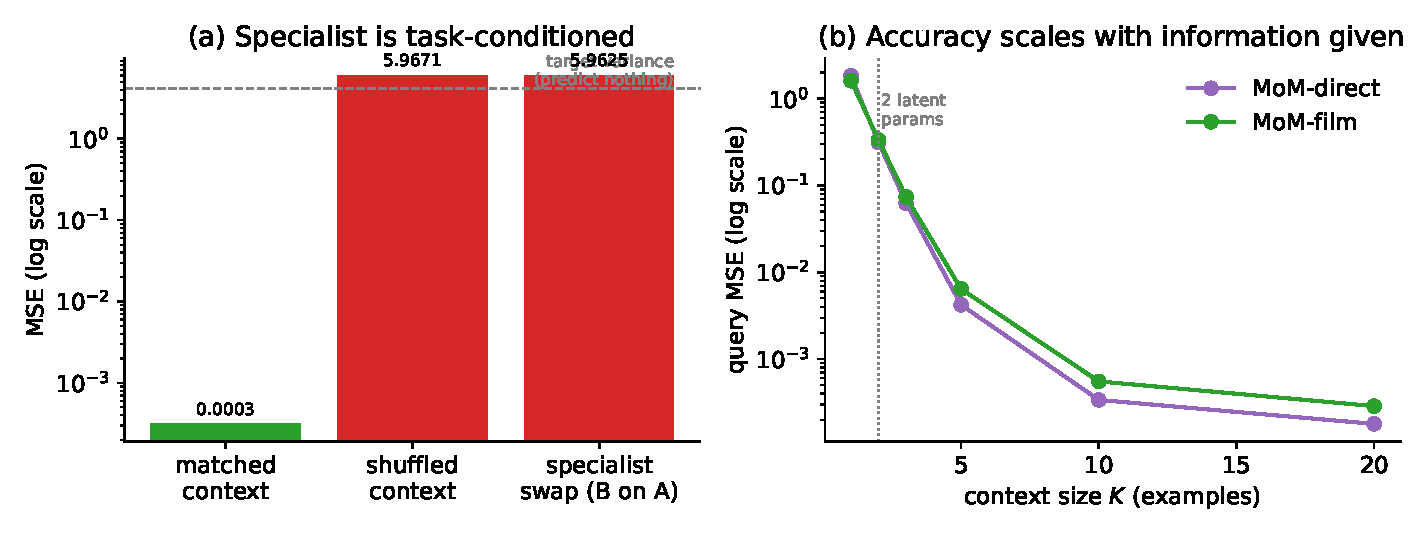
\includegraphics[width=\textwidth]{fig_ablation.pdf}
\caption{Mechanism ablations on the sinusoid MoM. (a) Replacing the context with
another task's examples, or running task $A$'s specialist on task $B$, raises error
$\sim$19{,}000$\times$---past the variance of predicting nothing---so the specialist
is fully context-determined. (b) Query error falls monotonically with context size
and resolves once $K$ exceeds the two latent task parameters: the encoder performs
inference, not retrieval.}
\label{fig:ablation}
\end{figure}

\subsection{Weight-space composition (candidate novelty)}\label{sec:compose}
If the encoder maps tasks to weights approximately linearly, emitted specialists
should compose. They do.
\begin{itemize}[leftmargin=1.4em]
  \item Interpolating two emitted specialists' weights
        $\theta=(1{-}\alpha)\theta_A+\alpha\theta_B$ tracks the blended target:
        \textbf{sinusoid} midpoint MSE 0.071 vs 6.03 task distance (85$\times$ below);
        \textbf{shapes} (a family \emph{not} closed under addition) 0.032 vs 0.695
        (22$\times$ below) --- coherent circle$\to$square morph (Fig.~\ref{fig:morph}).
  \item Emitted weight-space is approximately linear in the task latent $\Rightarrow$
        specialists compose algebraically; no in-context/MAML/PEARL baseline can
        interpolate task programs.
  \item \emph{Future work:} weight arithmetic ($A-B+C$) and whether composed
        specialists generalize to unseen task combinations.
\end{itemize}
\begin{figure}[h]\centering
\fbox{\parbox{0.9\textwidth}{\centering\vspace{1.2cm}
\texttt{exp22b\_morph.png} --- weight interpolation $\theta_{\text{circle}}\!\to\!
\theta_{\text{square}}$\\(purple = weight-blend output, gray = geometric target)
\vspace{1.2cm}}}
\caption{Specialists compose in weight space, even for a non-closed family.}
\label{fig:morph}
\end{figure}

\subsection{Scaling: does the in-context gap close?}\label{sec:scaling}
One might hope a one-pass adapter merely lags in-context attention at small scale and
catches up as the backbone grows. The opposite holds. As the enwik8 base grows from
$5$M to $15$M parameters the in-context gain itself grows
($0.163\!\to\!0.175$ bits/char), but the fraction MoM recovers \emph{shrinks}
($16\%\!\to\!11\%$; Table~\ref{tab:scaling}, Fig.~\ref{fig:scaling}). The $1$M point
is degenerate---in-context barely helps so weak a model, making the ratio
uninformative. The trend gives the thesis its upper boundary: for high-dimensional
sequence modeling, emission does not close the gap to attention, and the gap widens
with scale.
\begin{figure}[t]\centering
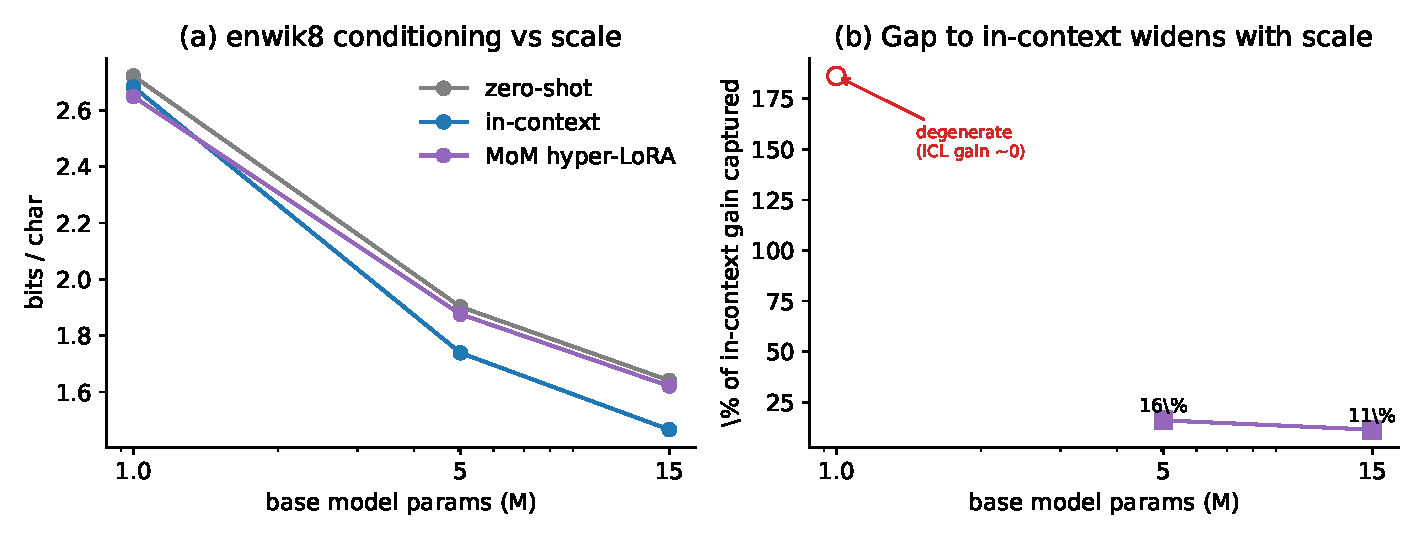
\includegraphics[width=\textwidth]{fig_scaling.pdf}
\caption{enwik8 scaling. (a) All three conditioning curves improve with base size,
but the MoM--in-context gap does not close. (b) The fraction of the in-context gain
captured by a one-pass emitted adapter shrinks from $16\%$ to $11\%$ over
$5\!\to\!15$M params; the $1$M point is degenerate (in-context gain $\approx0$).}
\label{fig:scaling}
\end{figure}
\begin{table}[h]\centering\small
\label{tab:scaling}
\begin{tabular}{lcccc}
\toprule
base size & zero-shot & in-context & hyper-LoRA & \% ICL gain captured \\
\midrule
1.0M & 2.722 & 2.683 & 2.649 & 186\%$^\ddagger$ \\
5.1M & 1.902 & 1.739 & 1.876 & 16\% \\
14.7M & 1.640 & 1.466 & 1.620 & 11\% \\
\bottomrule
\end{tabular}
\caption{enwik8. From 5M$\to$15M the in-context gain grows (0.163$\to$0.175) while
MoM's capture \emph{shrinks} (16\%$\to$11\%): the gap widens with scale.
$^\ddagger$1M degenerate (ICL gain only 0.039, ratio uninformative).}
\end{table}

%==================================================================
\section{Limitations}
Our experiments are at small scale---5--15M-parameter language models, MLP and
few-layer-transformer specialists, two consumer GPUs. We measure a scaling
\emph{trend}, but the absolute regime is small, and the language and ARC conclusions
should be read as bounds at this scale rather than at frontier scale. Emission fails
on high-dimensional and compositional tasks (language modeling, ARC), and on language
the failure \emph{grows} with scale, so the method is not a general-purpose substitute
for attention. Out of distribution, amortization extrapolates gracefully under
scaling shifts but breaks under structural shifts and is confidently wrong rather than
abstaining---a safety-relevant failure mode for deployment. Finally, weight-space
composition is demonstrated on synthetic families; whether emitted specialists for
real tasks compose as cleanly is open.

%==================================================================
\section{Conclusion}
Across six tasks and five domains we find a consistent pattern: emitting a
task-specific specialist dominates when the task family is low-dimensional and
amortizable---matching or beating gradient adaptation and the strongest amortized
baselines at far lower test-time cost---but cannot match in-context attention for
high-dimensional sequence modeling, where the gap widens with scale. The practical
decision rule that follows is simple: \emph{emit a specialist when the task family is
narrow and deployment cost matters; attend in-context when the task latent is rich,
especially at scale.} Two further findings sharpen the picture: mechanism ablations
show the emitted specialist is genuinely task-determined, and emitted specialists
compose algebraically in weight space---a property absent from the alternatives and a
promising direction for turning amortized emission from a conditioning trick into a
manipulable representation of tasks.

%==================================================================
\appendix
\section{Negative result: predicted gradients vs.\ local losses}
\label{app:negative}
This project began with a different question---whether a transformer could be trained
without global backpropagation by having each layer \emph{predict} its own incoming
gradient (a decoupled-neural-interfaces / synthetic-gradient
scheme~\citep{jaderberg2017dni})---and the negative result that emerged is worth
recording, both because it is clean and because it motivated the amortization view
that became MoM.

On a shape-classification task, per-token gradient predictors with RMS-normalized
targets and a bootstrapped target chain do train a small transformer with zero global
backward passes, reaching $96$--$99.6\%$ accuracy at two layers. But the approach has
two limits. First, it does not scale in depth: bootstrap error compounds and accuracy
collapses beyond a few layers \emph{unless} each stage is given an auxiliary local
loss that supplies an exact gradient anchor. Second---and this is the negative
result---once those local anchors are present, the gradient predictors are
\emph{redundant}: an ablation that removes them and keeps only the per-stage auxiliary
losses (greedy local learning,~\citealp{nokland2019local,belilovsky2019greedy})
matches end-to-end backpropagation ($100\%$ / $99.8\%$ at 4 / 6 layers on
classification; $0.0033$ vs.\ $0.0022$ MSE on autoregressive generation) while holding
peak training memory nearly flat in depth ($740$\,MB vs.\ backpropagation's $6927$\,MB
at 24 layers, a $9.4\times$ reduction).

A useful diagnostic emerged along the way: \emph{gradient predictability decays over
training}. The cosine similarity between a layer's true and predicted gradient is
$\approx0.99$ at initialization but drops sharply to roughly $0.2$--$0.5$ once the
loss converges, as gradients grow noisier and less structured. This weakens any
synthetic-gradient method in the late, low-loss regime and helps explain why such
methods help least exactly when one most wants a shortcut. The broader lesson---that
\emph{amortizing} a learned signal beats predicting a moving target---carried directly
into the specialist-emission framing of the main paper. This appendix could stand as a
short negative-results contribution on its own.

\section{Reproducibility}
All datasets are public: UCI HCV, UCI TCGA PAN-CAN RNA-seq, enwik8, ARC-AGI with the
RE-ARC procedural generators, and Gymnasium HalfCheetah-v5. All models are implemented
in PyTorch and trained on consumer GPUs (2$\times$NVIDIA~A2 and 2$\times$RTX~5070).
Code and configurations: \url{https://github.com/johnchowell/Model-of-Models}. Per-experiment settings are in
Table~\ref{tab:hparams}; results report multiple seeds where noted in
\S\ref{sec:exp} (sinusoid: 5; meta-RL: 3; tabular: 5-fold cross-validation).

\begin{table}[h]\centering\small
\setlength{\tabcolsep}{4pt}
\begin{tabular}{lp{0.62\textwidth}}
\toprule
Experiment & Key settings \\
\midrule
Sinusoid (\S5.1) & specialist MLP 1--40--40--1; encoder deep-sets, $d{=}128$; MoM
  $30$k steps, batch $256$, Adam lr $10^{-3}$ cosine; MAML $70$k meta-steps, batch
  $25$, inner lr $0.01$ ($1$ step), outer lr $10^{-3}$, 2nd-order; $K{=}10$. \\
Shapes (\S5.2) & specialist Fourier($t$)$+t$ $\to$ MLP, $1.7$k params (FiLM:
  $132$ mods); encoder transformer $d{=}128$; $8$k steps, batch $256$, lr $10^{-3}$;
  context $12$ points, curve length $32$. \\
Tabular (\S5.3) & few-shot net $d{=}128$ (genes) / row-encoder + FiLM head; $3$--$4$k
  steps, batch $32$--$64$, lr $10^{-3}$, wd $10^{-4}$; blood $K{=}16$ balanced,
  genes 5-way 5-shot, top-$1000$ genes; TabPFN v2 (PCA-$20$ for genes). \\
Meta-RL (\S5.4) & SAC, policy/critic hidden $256$; $300$ iters, batch $256$, lr
  $3{\times}10^{-4}$, $\gamma{=}0.99$, $\tau{=}5{\times}10^{-3}$; context encoder
  $z{\in}\mathbb{R}^{16}$, $64$ context transitions; episodes $200$ steps. \\
enwik8 (\S5.5) & base byte-LM $d{=}256$, $6$ layers, $T{=}768$, pretrain $8$k steps,
  batch $32$, lr $3{\times}10^{-4}$ OneCycle; hyper-LoRA rank $4$ on
  $\{o,\text{fc}_2\}$, $4$k steps; context $512$ bytes, target $256$. \\
ARC (\S5.6) & grid transformer, enc $4$ / dec $6$ layers, $d{=}256$, $12{\times}12$
  canvas; $60$k steps, batch $32$, lr $3{\times}10^{-4}$; $3$ example pairs; trained
  on RE-ARC, grids $\le 12{\times}12$. \\
Scaling (\S6.3) & bases $(d,L)\in\{(128,4),(256,6),(384,8)\}$; pretrain $6$k,
  hyper-LoRA $3$k steps each. \\
\bottomrule
\end{tabular}
\caption{Per-experiment configurations.}
\label{tab:hparams}
\end{table}

\bibliographystyle{plainnat}
\bibliography{references}

\end{document}
